\section{Results}
We have tested our implementation on a system comprising six slave nodes
against a centralized system making no RPCs. The distributed system was found
to take noticeably longer to handle a batch of bitmap queries of any given size
(\(0 \leq q \leq 1200\), where \(q\) is the number of queries) than the
centralized one. Figure~\ref{fig:graph-of-results} compares the execution time
of of the distributed system with that of the centralized system. It was found
that the distributed system had an execution time (in seconds) of
\(t_d(q) = 0.0045q + 0.07\) with \(R^2 = 0.9919\) while the centralized system
had an execution time (in seconds) of \(t_c(q) = 0.0002q - 0.0023\) with
\(R^2 = 0.9818\) (in both cases, \(q\) is the number of queries, as stated
above). Since the slope of \(t_d(q)\) surpasses the slope of \(t_c(q)\) we
expect the distributed system to perform much more slowly. This is an expected
result due to the time required to perform RPCs and execute the query planner.
Despite the slower performance, using a distributed system provides fault
tolerance. Further, while a centralized system cannot be altered to provide
fault tolerance, the execution time of the distributed system could be improved
through furtehr optimization.
%
\begin{figure}
    \centering
    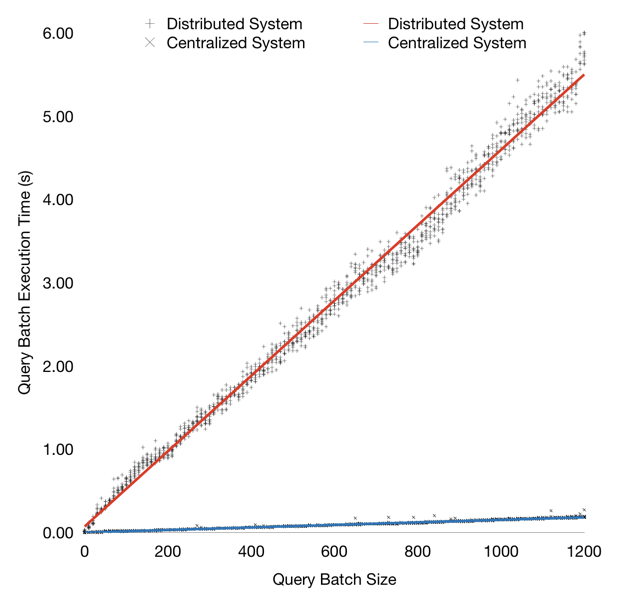
\includegraphics[width=\columnwidth]{query-experiment-results}
    \caption{Query experiment results.}\label{fig:graph-of-results}
\end{figure}
